\chapter{Contact Planの臨時更新の天体内への限定的な拡散の提案}
\label{chap:suggestion}
\ref{section:ContactPlanの臨時更新の課題}節で述べたとおり, 
Contact Planの臨時更新には配送遅延の低下度合いと拡散による運用面における影響によって対象を選定することが必要である. 
Bezirgiannidisらの提案した全てのノードにおいて臨時更新を行う既存手法に対して, 
本論文ではこの課題に対して, Contactの失敗が起きた際に, 
その通知を行いContact Planを更新するノードを
天体内のノードにのみ拡散し, 他天体のノードには拡散しない手法を提案する. 
本章ではこの提案が満たすべき要件について整理し, 
それらに対する既存手法と提案手法の定性的な特性について述べる. 

\section{要件1:臨時更新による配送遅延の低下}
\label{section:要件1}
\ref{section:ContactPlanの臨時更新}で述べたように, 
Contact Planの臨時更新の目的は, 想定されたContactに失敗した場合にその
情報をDTNの他のノードに拡散しContact Planを更新することで,
DTNの各ノードが最新のトポロジーを認識し配送遅延の増加を抑えることである. 
既存手法と提案手法の効果について表\ref{fig:experimentation_topology}の例を用いて考える.

\begin{figure}[tbh]
    \centering
    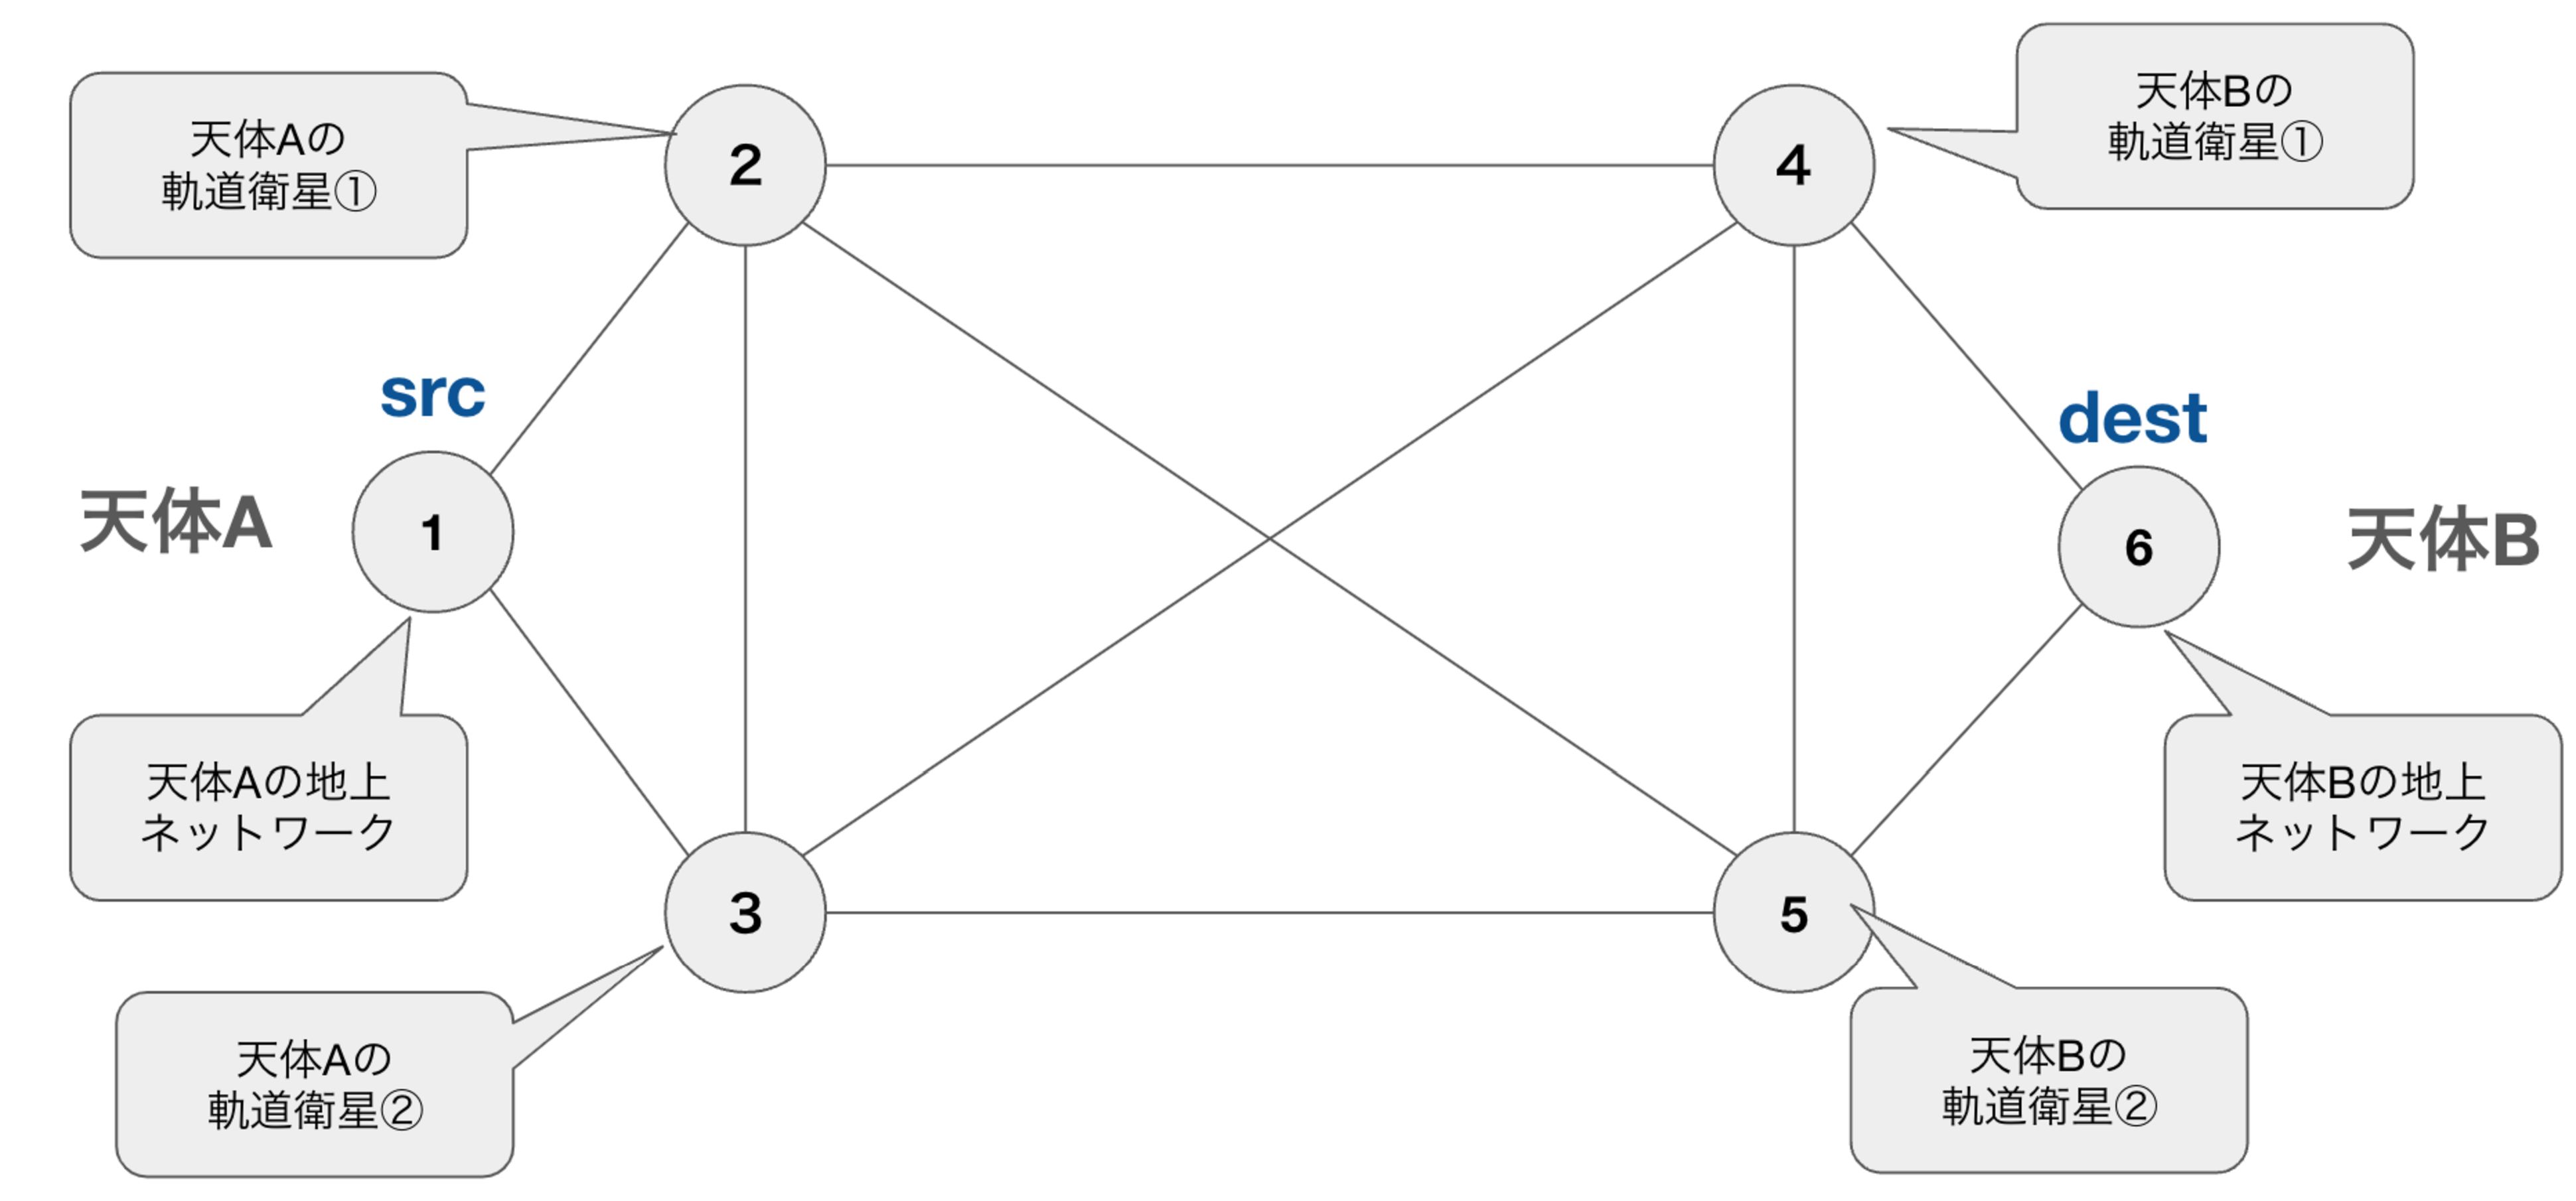
\includegraphics[width=0.7\textheight]{img/thesis_Sample_topology.pdf}
    \caption{本実験で用いるトポロジー}
    \label{fig:experimentation_topology}
    \begin{minipage}{\textwidth}
        \raggedright
        \vspace{3mm}
        \fontsize{10pt}{12pt}\selectfont
        ノード1は天体Aの地上DTNネットワークを代表したノード, ノード2とノード3は
        天体Aの軌道上に存在する宇宙のDTNノード, ノード4とノード5は
        天体Bの軌道上に存在する宇宙のDTNノード, 
        ノード6は天体Bの地上DTNネットワークを代表したノードを示す. 
    \end{minipage}
\end{figure}

ノード1から3は天体A, ノード4から6はそれぞれ天体Bに属するDTNノードであり, 
ノード1と6はそれぞれの地表DTNのノード, ノード2から5はそれぞれの天体の軌道上にある
宇宙のDTNノードである. 
このトポロジーにおいて, 今ベストパスがノード1-2-4-6の経路(経路1)であるとし, 仮に
ノード4から6のContactが何らかの理由で失敗した場合に, ベストパスはノード1-2-5-6の経路(経路2)となり, 
ただしこれよりは最適経路ではないもののノード1-2-4-5-6の経路(経路3)でもバンドルの配送が可能であるとする.

既存手法も提案手法も用いず更新を行わない場合, どのノードもそのContactの失敗を知らないため
すべてのノードはベストパスが経路1のままと認識し, ノード4においてノード6へのバンドルの配送を試み続ける.
TTLの期限切れまでそれを試み続け, そのContactの復旧が起きた場合にのみBundleの送信が成功する. 

既存手法では, その情報をノード4を起点に発信し, その情報を受け取ったノードは順次Contact Planから
当該Contactを削除し, Contact Planを更新する. これにより, 失敗発生直後よりノード4は代替経路となる経路3を
利用することが可能になり, 到達遅延は増加するものの, Bundleの送信には成功する. さらにこの場合, 
天体間遅延を超えてこの情報が天体Aのノード1・2・3に配信されると, 
ノード2は経路2が最適経路と認識することができるようになり, 配送遅延を低下させることができる. 

提案手法では, 当初は既存手法同様経路3をすぐに利用できるようになるが, 
天体間には更新情報を伝搬しないため経路2が利用されることはなく, 
失敗したContactの終了または復旧まで経路1を利用することができない. 

ただし経路2と経路3の遅延の差はノード2からノード4の遅延とノード2からノード5の遅延の差, 
すなわち天体Bの2つの衛星の天体Aの衛星との距離の差によるものである. 
これは天体間の距離に対して基本的には小さいものであると考えられ, 既存手法で途中から経路2を利用できることの
利点は非常に限定的であり, 配送遅延の低下という点に置いて提案手法の有効性は既存手法に
対して大きな差異があるとは言えないと予想される. 

\begin{figure}[tbh]
    \centering
    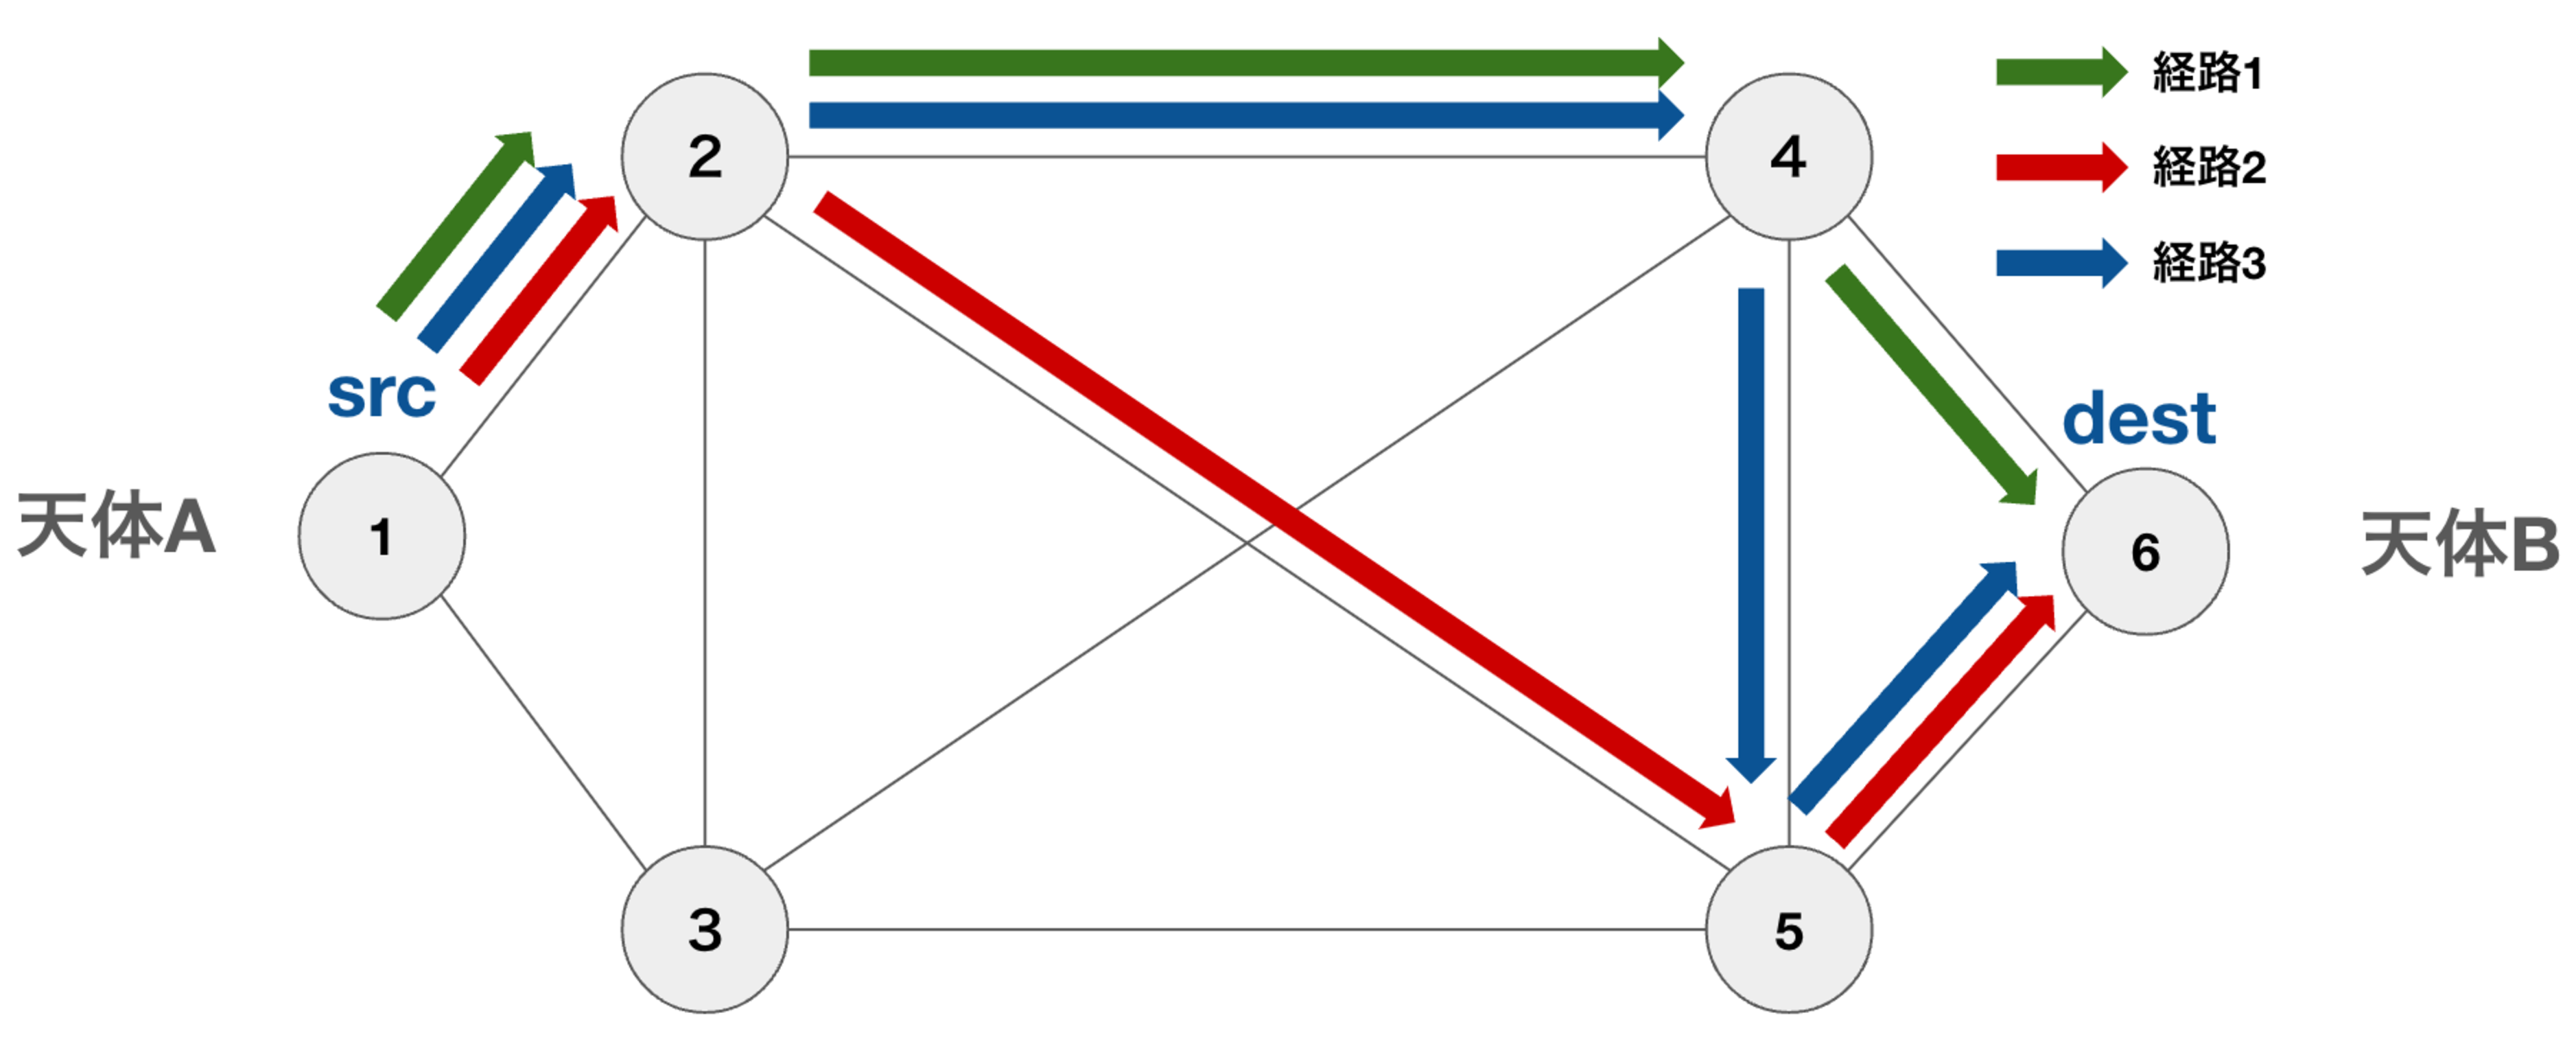
\includegraphics[width=0.7\textheight]{img/example_of_routechange.pdf}
    \caption{既存手法と提案手法において選択される代替経路の例}
    \label{fig:example_of_routechange}
    \begin{minipage}{\textwidth}
        \raggedright
        \vspace{3mm}
        \fontsize{10pt}{12pt}\selectfont
    \end{minipage}
\end{figure}

\section{要件2:臨時更新による運用面での効果}
\label{section:要件2}
\ref{section:要件1}で述べたように, Contact Planの臨時更新を
もし天体間においても行う場合, 貴重な天体間のリンクを消費することになる.
提案手法はこの点において, 既存手法と違い自天体内のノードにのみ拡散するため, 
この消費を行わない. 既存手法のCPUPにおける更新メッセージのProtocol Data Unit(PDU)は
表\ref{table:cpup_pdu_format}のようになっており, このPDU内で示される
Command Blockのフォーマットは表\ref{table:command_block_format}のようになっている.
このPDUを用いて全てのノードに対して臨時更新を行う場合, そのサイズ分
天体間のリンクを消費する.

\begin{table}[htbp]
    \centering
    \caption{既存手法におけるCPUPのPDUのフォーマット}
    \label{table:cpup_pdu_format}
    \begin{tabular}{|c|c|c|c|}
      \hline
      Byte 0 & Byte 1 & Byte 2 & Byte 3 \\
      \hline
      \multicolumn{1}{|c|}{Version num.} & \multicolumn{3}{c|}{Number of Command Blocks (SDNV)} \\
      \hline
      Byte 4 & Byte 5 & Byte 6 & Byte 7 \\
      \hline
      \multicolumn{4}{|c|}{1\textsuperscript{st} Command Block} \\
      \hline
      \multicolumn{4}{|c|}{...} \\
      \hline
      Byte $4\times n$ & Byte $4\times n+1$ & Byte $4\times n+2$ & Byte $4\times n+3$ \\
      \hline
      \multicolumn{4}{|c|}{$n$\textsuperscript{th} Command Block} \\
      \hline
    \end{tabular}
    \begin{minipage}{\textwidth}
        \centering
        \vspace{3mm}
        参考文献\cite{Bezirgiannidis2013}Table1より引用.  
    \end{minipage}
  \end{table}
\begin{table}[htbp]
    \centering
    \caption{既存手法におけるCPUPのCommand Blockのフォーマット}
    \label{table:command_block_format}
    \begin{tabular}{|c|c|c|c|}
      \hline
      Byte 0 & Byte 1 & Byte 2 & Byte 3 \\
      \hline
      \multicolumn{2}{|c|}{Creation Timestamp (SDNV)} & \multicolumn{2}{c|}{Command Expiry (SDNV)} \\
      \hline
      Byte 4 & Byte 5 & Byte 6 & Byte 7 \\
      \hline
      \multicolumn{3}{|c|}{Command Originator (SDNV)} & Command Type \\
      \hline
      Byte 8 & Byte 9 & ... & Byte $n$ \\
      \hline
      \multicolumn{2}{|c|}{Command Parameter 1 (SDNV)} & \multicolumn{1}{c|}{...} & Comm. Param. $k$ (SDNV) \\
      \hline
    \end{tabular}
    \begin{minipage}{\textwidth}
        \centering
        \vspace{3mm}
        参考文献\cite{Bezirgiannidis2013}Table2より引用.  
    \end{minipage}
  \end{table}
  